\chapter[Residence time]{Time of residence in states\\[0.5cm] Introduction to
compartmental models}
\label{chap:residence_time}


\section{Time spent in a state -- Some probability theory}
\label{sec:residence_time}
We suppose that a system/object/individual can be in two states $S_1$ and $S_2$.
These states can be anything:
\begin{itemize}
\item $S_1$: working, $S_2$: broken,
\item $S_1$: infected, $S_2$: recovered,
\item $S_1$: alive, $S_2$: dead.
\end{itemize}
At time $t=0$, the system is in state $S_1$.
An event happens at some time $t=\tau\geq 0$, which triggers the switch from state $S_1$ to state $S_2$. Suppose that we are able to conduct an experiment with infinitely many copies of this system, and are interested in obtaining some type of description of the time it takes for the system to switch states.

Let us reformulate this problem in the language of probability theory.
A \textbf{random variable} is a variable that takes random values, that is, a mapping from random experiments to numbers. 
Here, let us call $T$ the random variable ``time spent in state $S_1$ before switching into state $S_2$''. 
We take a collection of objects or individuals that are in state $S_1$ and want some law for the \textbf{distribution} of the times spent in $S_1$, i.e., a law for $T$.
For example, we make light bulbs and would like to tell our customers that on average, our light bulbs last 200 years.
For this, we conduct an \textbf{infinite} number of experiments, and observe the time that it takes, in every experiment, to switch between $S_1$ and $S_2$.
From this, we deduce a model, which in this context is called a \textbf{probability distribution}.

Before we proceed any further, let us make one remark here. Roughly speaking, probability theory assumes that it is indeed possible to carry out an infinite number of experiments. Statistics, on the other hand, deals with the use of probability theory in ``real life'', where the number of experiments is intrinsically limited.

\begin{figure}[htbp]
\begin{center}
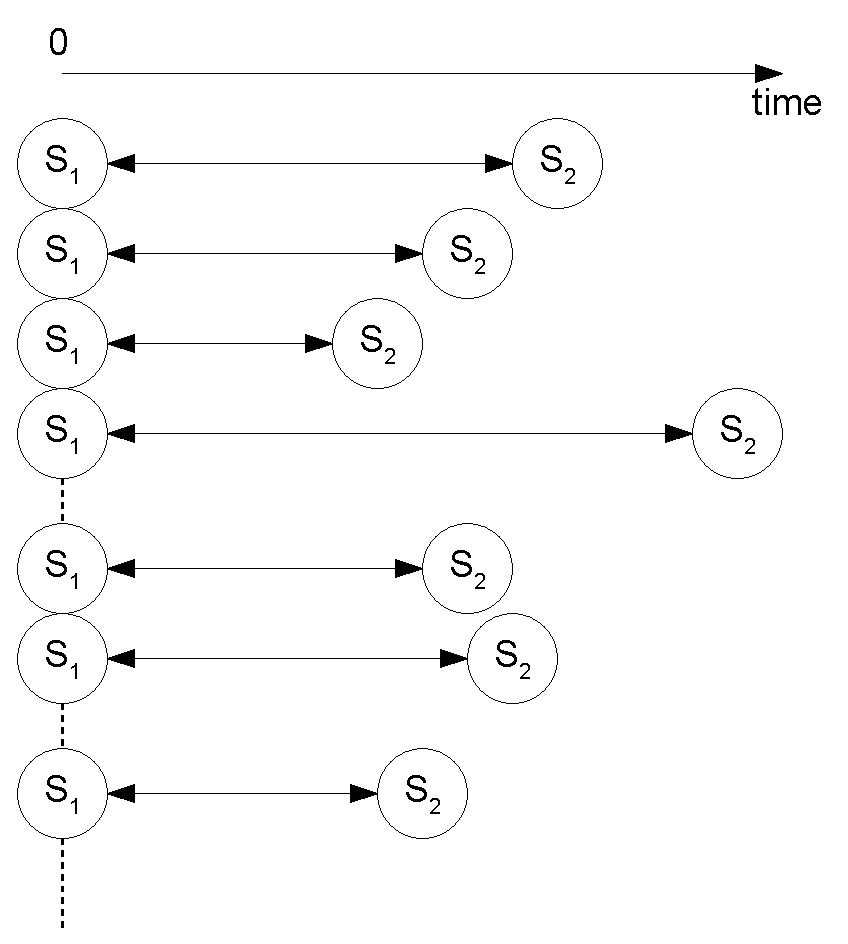
\includegraphics[height=0.45\textwidth]
{../figs_03_residence_time/random_length_sample}
\caption{Time until the switch from state $S_1$ to state $S_2$, for several experiments. From this, we could deduce a distribution for the time of sojourn in state $S_1$.}
\end{center}
\end{figure}

Returning to the time spent in a state, we assume that $T$ is a \textbf{continuous} random variable, that is, $T$ takes continuous values. Examples of continuous random variables are the height or age of a person (if measured very precisely), distances, times, etc.
Another type of random variables are \textbf{discrete} random variables, which take values in a denumerable set: heads or tails on a coin toss, the number rolled on a dice, the height of a person, if expressed rounded without subunits, the age of a person in years (without subunits), etc.

A \textbf{probability} is a function $\mathcal{P}$, from a probability space to $[0,1]$.
Formally: $(\Omega,\mathcal{F},\mathcal{P})$ is a probability space, with $\Omega$ the \textbf{sample} space, $\mathcal{F}$ a $\sigma$-algebra of subsets of $\Omega$ whose elements are the \textbf{events}, and $\mathcal{P}$ a \textbf{measure} from $\mathcal{F}$ to $[0,1]$ such that $\mathcal{P}(E)\geq 0$, $\forall E\subset\Omega$, $\mathcal{P}(\Omega)=1$ and $\mathcal{P}(E_1\cup E_2\cup\cdots)=\sum_i\mathcal{P}(E_i)$.

A probability gives the likelihood of an event occurring, among all the events that are
possible, in that particular setting. For example, 
\[
\Proba{\textrm{getting heads
when tossing a coin}}=1/2
\]
and 
\[
\Proba{\textrm{getting tails when tossing a
coin}}=1/2.
\]
Since $T$ is continuous, it has a continuous \textbf{probability density function} (p.d.f.), $f$, which satisfies:
\begin{itemize}
\item $f\geq 0$,
\item $\int_{-\infty}^{+\infty}f(s)ds=1$.
\item $\Proba{a\leq T\leq b}=\int_a^bf(t)dt$.
\end{itemize}
\begin{figure}[htbp]
\begin{center}
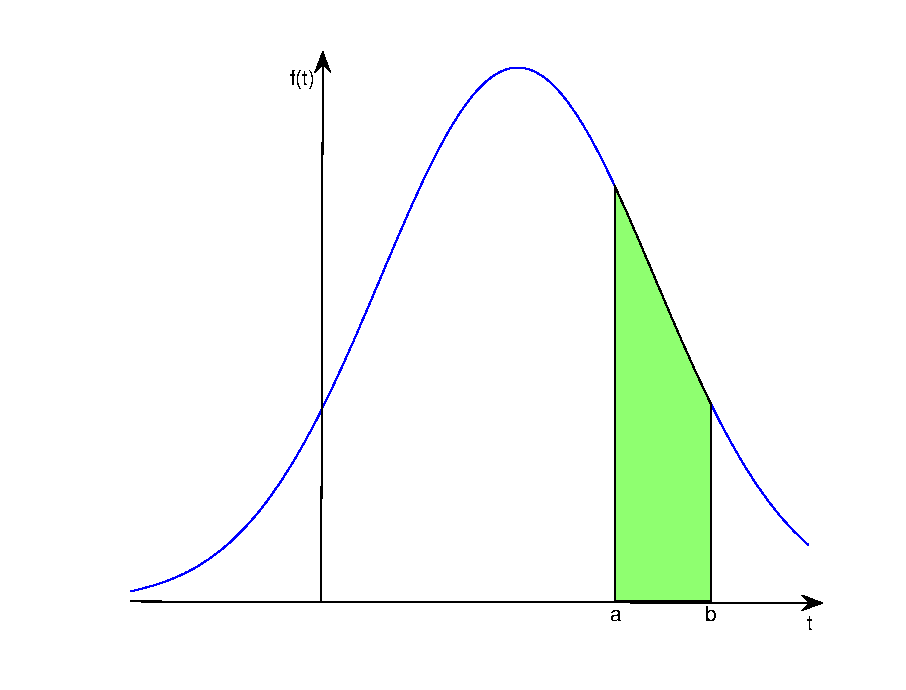
\includegraphics[width=0.5\textwidth]{../figs_03_residence_time/distrib_a_b}
\caption{A continuous probability distribution function (curve) and $\Proba{a\leq T\leq b}$ (area).}
\end{center}
\end{figure}
The \textbf{cumulative distribution function} (c.d.f.) is a function $F(t)$ that characterizes the distribution of $T$, and defined by
\[
F(s)=\Proba{T\leq s}=\int_{-\infty}^sf(x)dx.
\]
\begin{figure}[htbp]
\begin{center}
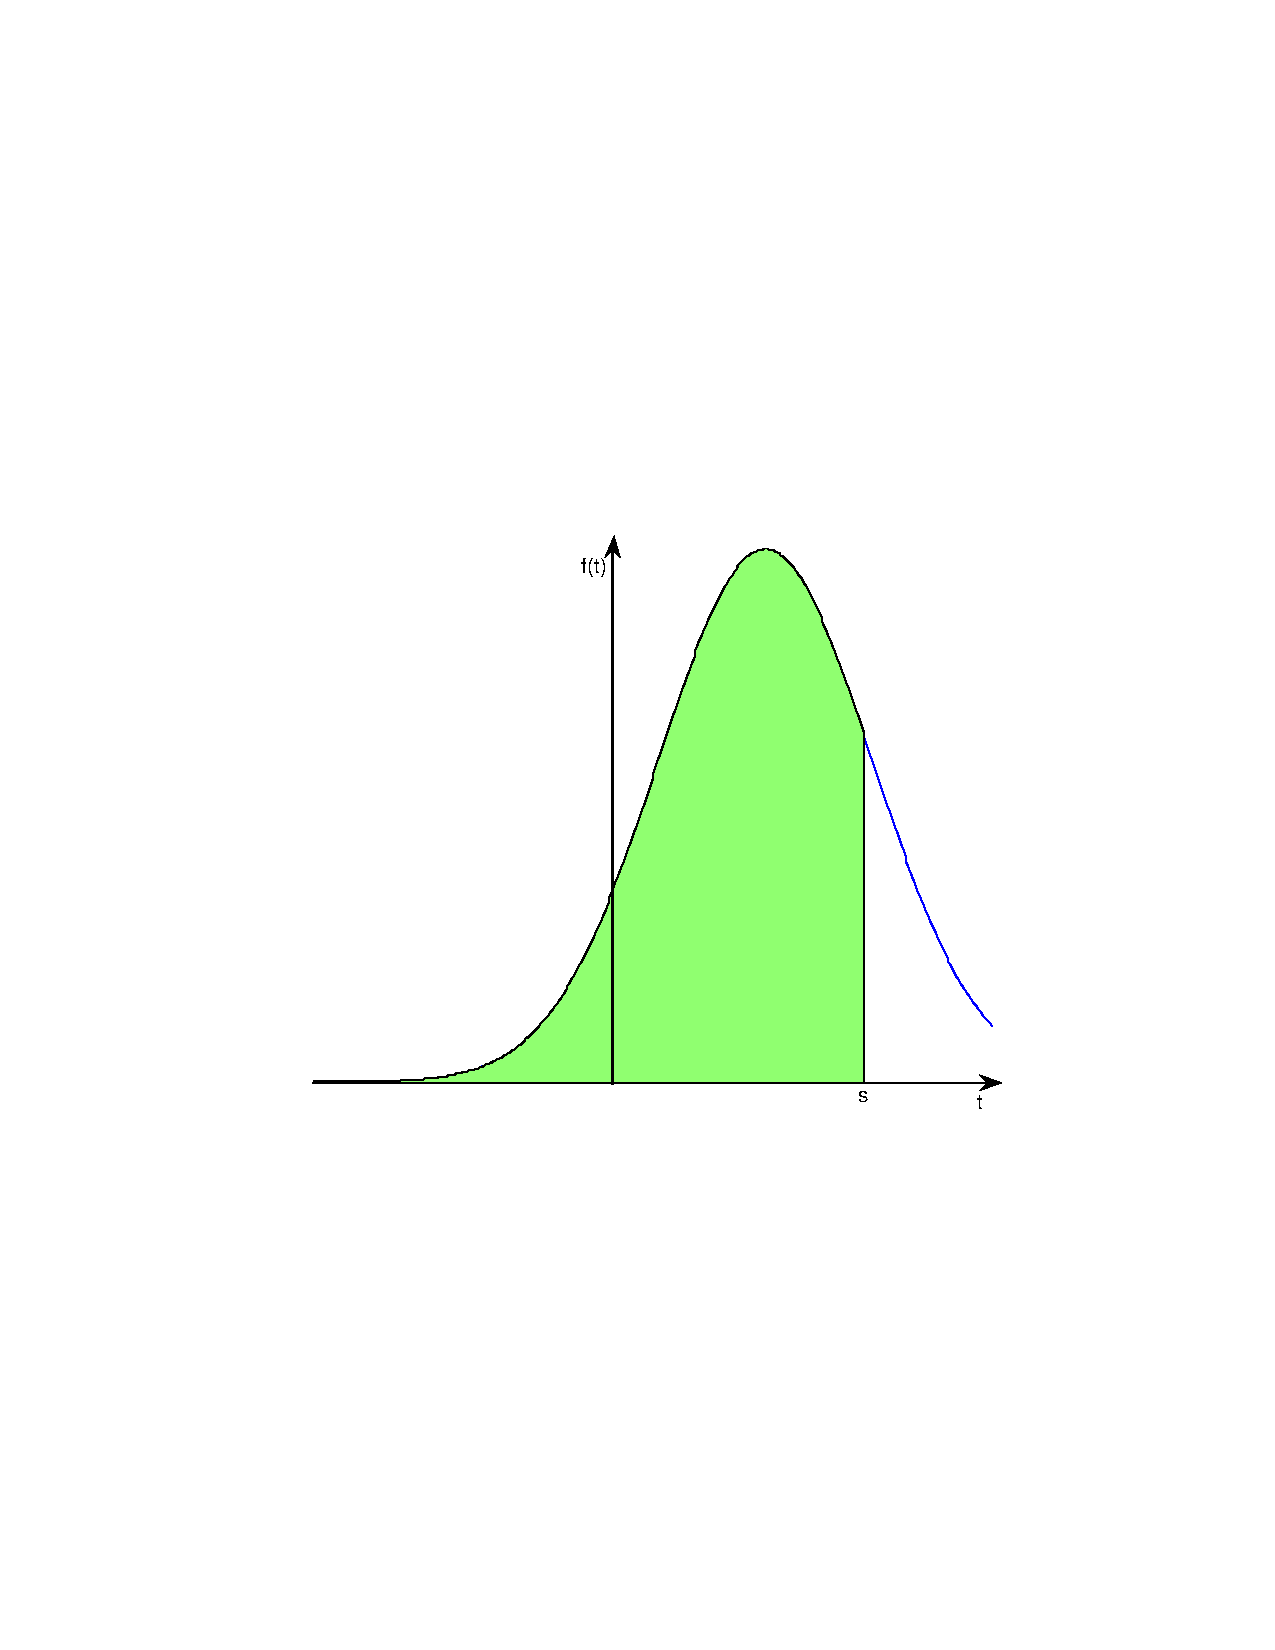
\includegraphics[width=0.45\textwidth]{../figs_03_residence_time/cdf_auc}
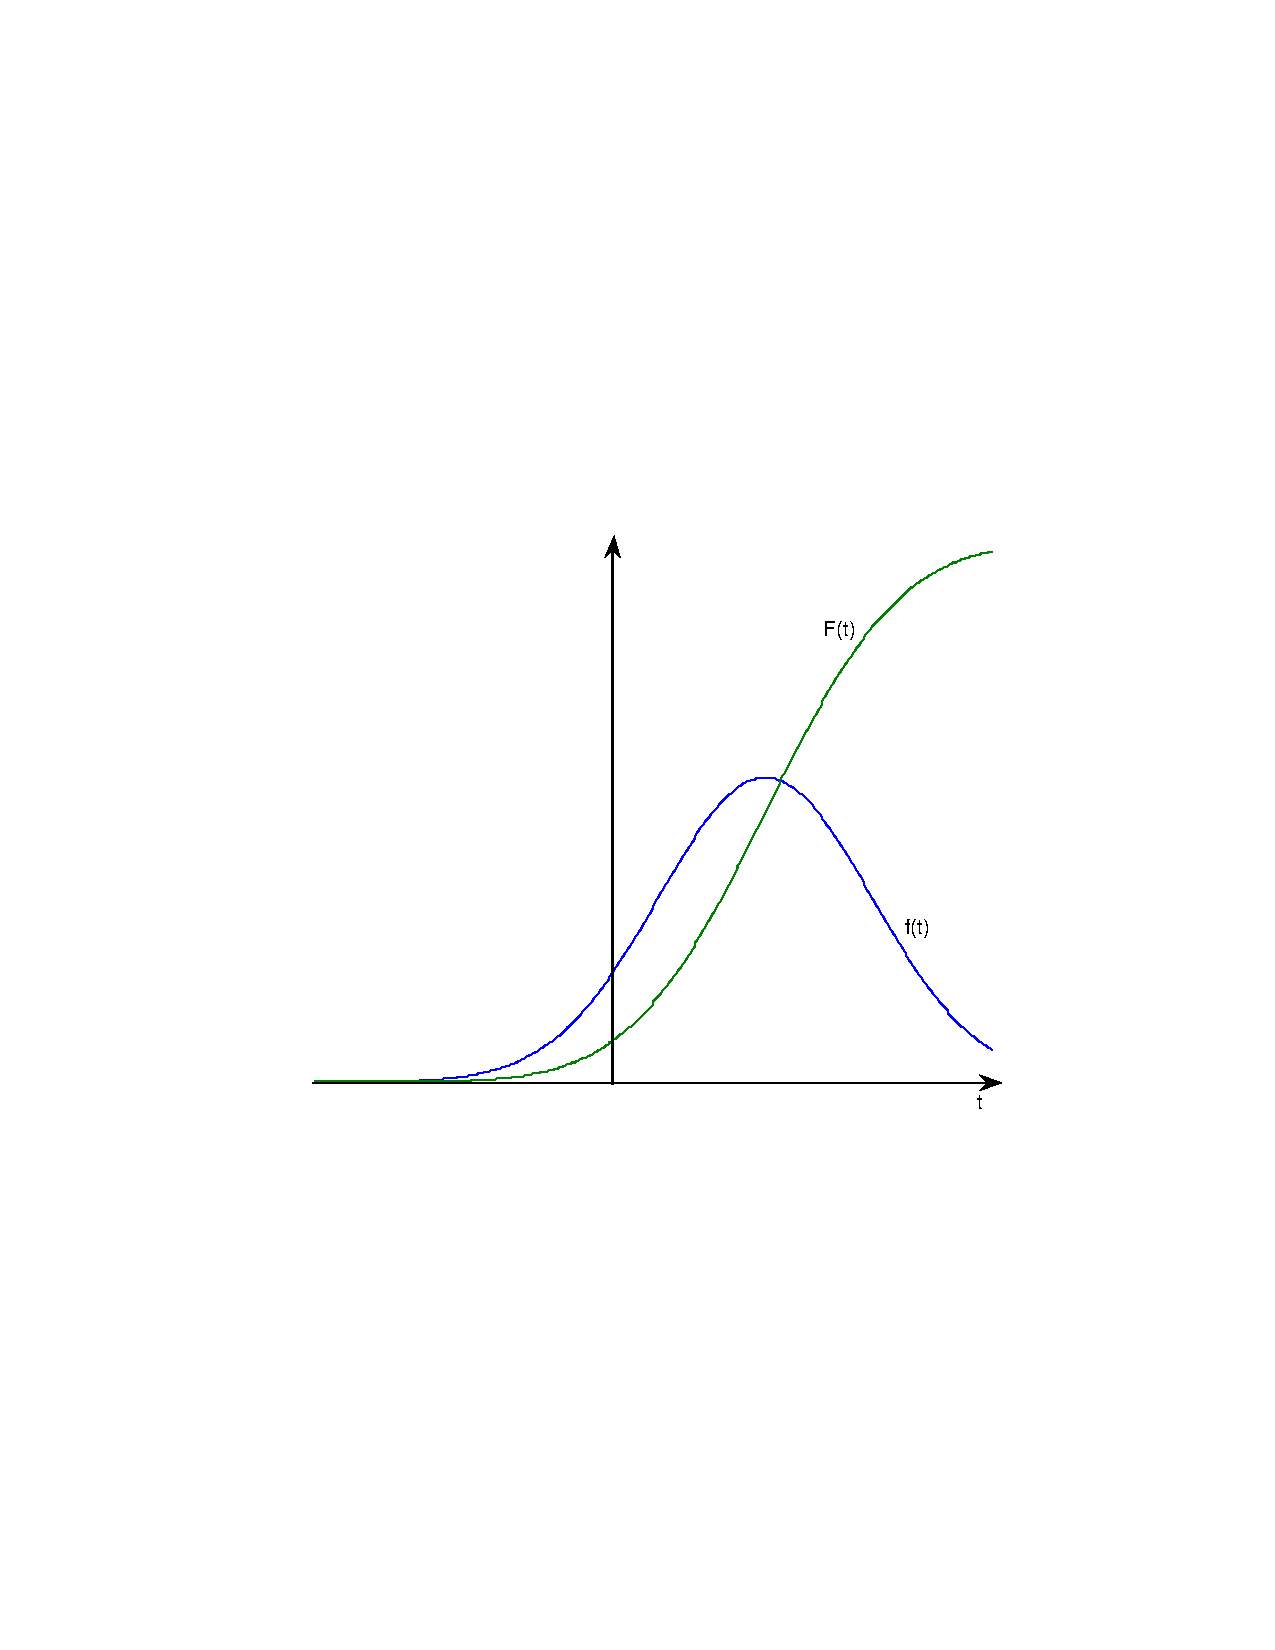
\includegraphics[width=0.45\textwidth]{../figs_03_residence_time/cdf_plot}
\caption{The link between the cumulative distribution function and the probability density function. The integral from $-\infty$ to $t$, shown on the left by the area under the curve $f$, gives a function $F(t)$ (right).}
\label{fig:cum_distrib}
\end{center}
\end{figure}
\begin{itemize}
\item
Since $f$ is a nonnegative function, $F$ is nondecreasing.
\item
Since $f$ is a probability density function, $\int_{-\infty}^{+\infty}f(s)ds=1$, and thus $\lim_{t\to\infty}F(t)=1$.
\end{itemize}
\begin{figure}[htbp]
\begin{center}
\end{center}
\end{figure}

For a continuous random variable $T$ with probability density function $f$, the \textbf{mean} value of $T$, denoted $\bar T$ or $E(T)$, is given by
\[
E(T)=\int_{-\infty}^{+\infty} tf(t)dt.
\]
Another characterization of the distribution of the random variable
$T$ is through the \textbf{survival} (or \textbf{sojourn}) function. 
The survival function of state $S_1$ is given by 
\begin{equation}
  \S(t)=1-F(t)=\Proba{T>t}
  \label{eq:survival}
\end{equation}
This gives a description of the \textbf{sojourn time} of a
system in a particular state (the time spent in the state).
$\S$ is a nonincreasing function (since $\S=1-F$
with $F$ a c.d.f.), and
$\S(0)=1$ (since $T$ is a positive random variable).
The \textbf{average sojourn time} $\tau$ in state $S_1$ is given by
\[
\tau=E(T)=\int_0^\infty tf(t)dt
\]
Assuming that $\lim_{t\to\infty}t\S(t)=0$ (which is verified
for most probability distributions), 
\[
\tau=\int_0^\infty \S(t)dt.
\]



\section{The exponential distribution}

The random variable $T$ has an \textbf{exponential} distribution if its probability density function takes the form
\begin{equation}\label{eq:exp_distrib}
f(t)=\begin{cases}0&\textrm{if }t<0,\\
\theta e^{-\theta t}&\textrm{if }t\geq 0,
\end{cases}
\end{equation}
with $\theta>0$. Then the
survival function for state $S_1$ is of the form $\S(t)=e^{-\theta
  t}$, for $t\geq 0$, and the average sojourn time in state $S_1$ is
\[
\tau=\int_0^\infty e^{-\theta t}dt=\frac 1\theta
\]
If on the other hand, for some constant $\omega>0$,
\[
\S(t)=
\left\{
\begin{array}{ll}
1, & 0\leq t\leq\omega \\
0, & \omega<t
\end{array}
\right.
\]
which means that $T$ has a Dirac delta distribution
$\delta_\omega(t)$, then the average sojourn time is a constant, namely
\[
\tau=\int_0^\omega dt=\omega
\]
These two distributions can be regarded as extremes.



\section{A cohort model} 
We consider a population consisting of individuals born at the same time (a \textbf{cohort}), for example, the same year.
We suppose
\begin{itemize}
\item At time $t=0$, there are initially $N_0>0$ individuals.
\item All causes of death are compounded together. 
\item The time until death, for a given individual, is a random variable $T$, with continuous probability density distribution $f(t)$ and survival function $P(t)$.
\end{itemize}
Denote $N(t)$ the population at time $t\geq 0$. Then
\begin{equation}\label{eq:N_general}
N(t)=N_0P(t).
\end{equation}
\begin{itemize}
\item $N_0P(t)$ gives the proportion of $N_0$, the initial population, that is still alive at time $t$.
\end{itemize}

\paragraph{Case where $T$ is exponentially distributed}
Suppose that $T$ has an exponential distribution with mean $1/d$ (or parameter $d$), $f(t)=de^{-dt}$. Then the survival function is $P(t)=e^{-dt}$, and \eqref{eq:N_general} takes the form
\begin{equation}\label{eq:N}
N(t)=N_0e^{-dt}.
\end{equation}
Now note that
\begin{align*}
\frac{d}{dt} N(t) &= -dN_0e^{-dt} \\
&= -dN(t),
\end{align*}
with $N(0)=N_0$.
Thus, the ODE $N'=-dN$ makes the assumption that the life expectancy at birth is exponentially distributed.


\paragraph{Case where $T$ has a Dirac delta distribution}
Suppose that $T$ has a Dirac delta distribution at $t=\omega$, giving the survival function 
\[
P(t)=\begin{cases}
1, & 0\leq t\leq\omega,\\
0, & t>\omega.
\end{cases}
\]
Then \eqref{eq:N_general} takes the form
\begin{equation}\label{eq:N2}
N(t)=\begin{cases}
N_0, & 0\leq t\leq\omega,\\
0, & t>\omega.
\end{cases}
\end{equation}
All individuals survive until time $\omega$, then they all die at time $\omega$.
Here, we have $N'=0$ everywhere except at $t=\omega$, where it is undefined.



\section{Sojourn times in an SIS disease transmission model} 
\label{sec:epid_residence_time}
The population can be 
\begin{itemize}
\item closed (no immigration, no emigration, birth and death are neglected). 
\item open
\item homogeneous and homogeneously mixed (or not)
\end{itemize}
The population has a structure
\begin{itemize}
\item classification of individuals according to their disease status
\begin{itemize}
\item susceptible (S): individuals not infective but who are capable of contracting the disease
\item latent or exposed (E): infected by the disease, but not yet infectious
\item infective (I): infectious individual; an individual can be infectious before symptoms appear.
\item removed (R): no longer infectious, whether by acquiring immunity or death...
\item carrier: in some diseases, individual can remain infectious for long periods (e.g. for life), but do not show any symptoms of the disease themselves.
\end{itemize}
\item age
\item sex
\end{itemize}
Types of models
\begin{itemize}
\item SI model: no recovery.
\item SIS model: recovery but no immunity.
\item SIR model: recovery with permanent immunity.
\item SIRS model: recovery with temporary immunity.
\item ...
\end{itemize}




Consider a disease and a a population of individuals who can be infected by this disease.
Both can be anything: a human population subject to influenza, an animal population subject to foot and mouth disease, a rumor spreading in a human population, inovation spreading through businesses,
a computer virus spreading on the internet..

Suppose that individuals can be identified with respect to their epidemiological status:
\begin{itemize}
\item susceptible to the disease,
\item infected by the disease,
\item recovered from the disease.
\end{itemize}
These states are clearly of the type we were discussing in Section~\ref{sec:residence_time}.
To be more specific, consider a disease that confers no immunity. In this case,
individuals are either
\begin{itemize}
\item \textbf{susceptible} to the disease, with the number of such individuals at time $t$ denoted by $S(t)$,
\item or \textbf{infected} by the disease (and are also \textbf{infective} in the sense that they propagate the disease), with the number of such individuals at time $t$ denoted by $I(t)$.
\end{itemize}
We want to model the evolution with time of $S$ and $I$ ($t$ is omitted unless
necessary).
{\bf Extremely important:} State all your hypotheses.


\paragraph{Hypotheses}
\begin{itemize}
\item Individuals typically recover from the disease.
\item The disease does not confer immunity.
\item There is no birth or death.
\item Infection is of \textbf{standard incidence} type
\end{itemize}
Once your hypotheses are stated, detail them if need be.


\subsection*{Recovery and No immunity}
Individuals recover from the disease: the infection is not permanent.
Upon recovery from the disease, an individual becomes susceptible again
immediately.
Good description for diseases that confer no immunity, e.g., the cold or gonorrhea.

\paragraph{No birth or death}
Suppose that
\begin{itemize}
\item the time period of interest is short,
\item the population is large enough,
\end{itemize}
then it is reasonable to assume that the total population is constant, in the absence of disease.

For mild diseases (cold, etc.), there are very little risks of dying from the
disease. We assume no disease-induced death.

Hence $N\equiv N(t)=S(t)+I(t)$ is the (constant) total population.


\paragraph{Standard incidence}
New infectives result from random contacts between susceptible and infective individuals, described using standard incidence:
\[
\beta\frac{SI}{N},
\]
\begin{itemize}
\item $\beta SI/N$ is a rate (per unit time), 
\item $\beta$ is the \textbf{transmission coefficient}, giving probability of transmission of the disease in case of a
contact, times the number of such contacts made by an infective per
unit time.
\end{itemize}


\frame{\frametitle{Recovery}
We have not yet stated our hypotheses on the recovery process..
Traditional epidemiological models assume recovery from disease
with a rate constant $\gamma$.
Here, assume that, of the individuals who have become infective at time $t_0$, a
fraction $P(t-t_0)$ remain infective at time $t\geq t_0$. 
Thus, considered for $t\geq 0$, the function $P(t)$ is a survival
function.
}

Figure~\ref{fig:flow_diagram_SIS_P} is a \textbf{flow diagram} of our model.
\begin{figure}[htbp]
\begin{center} 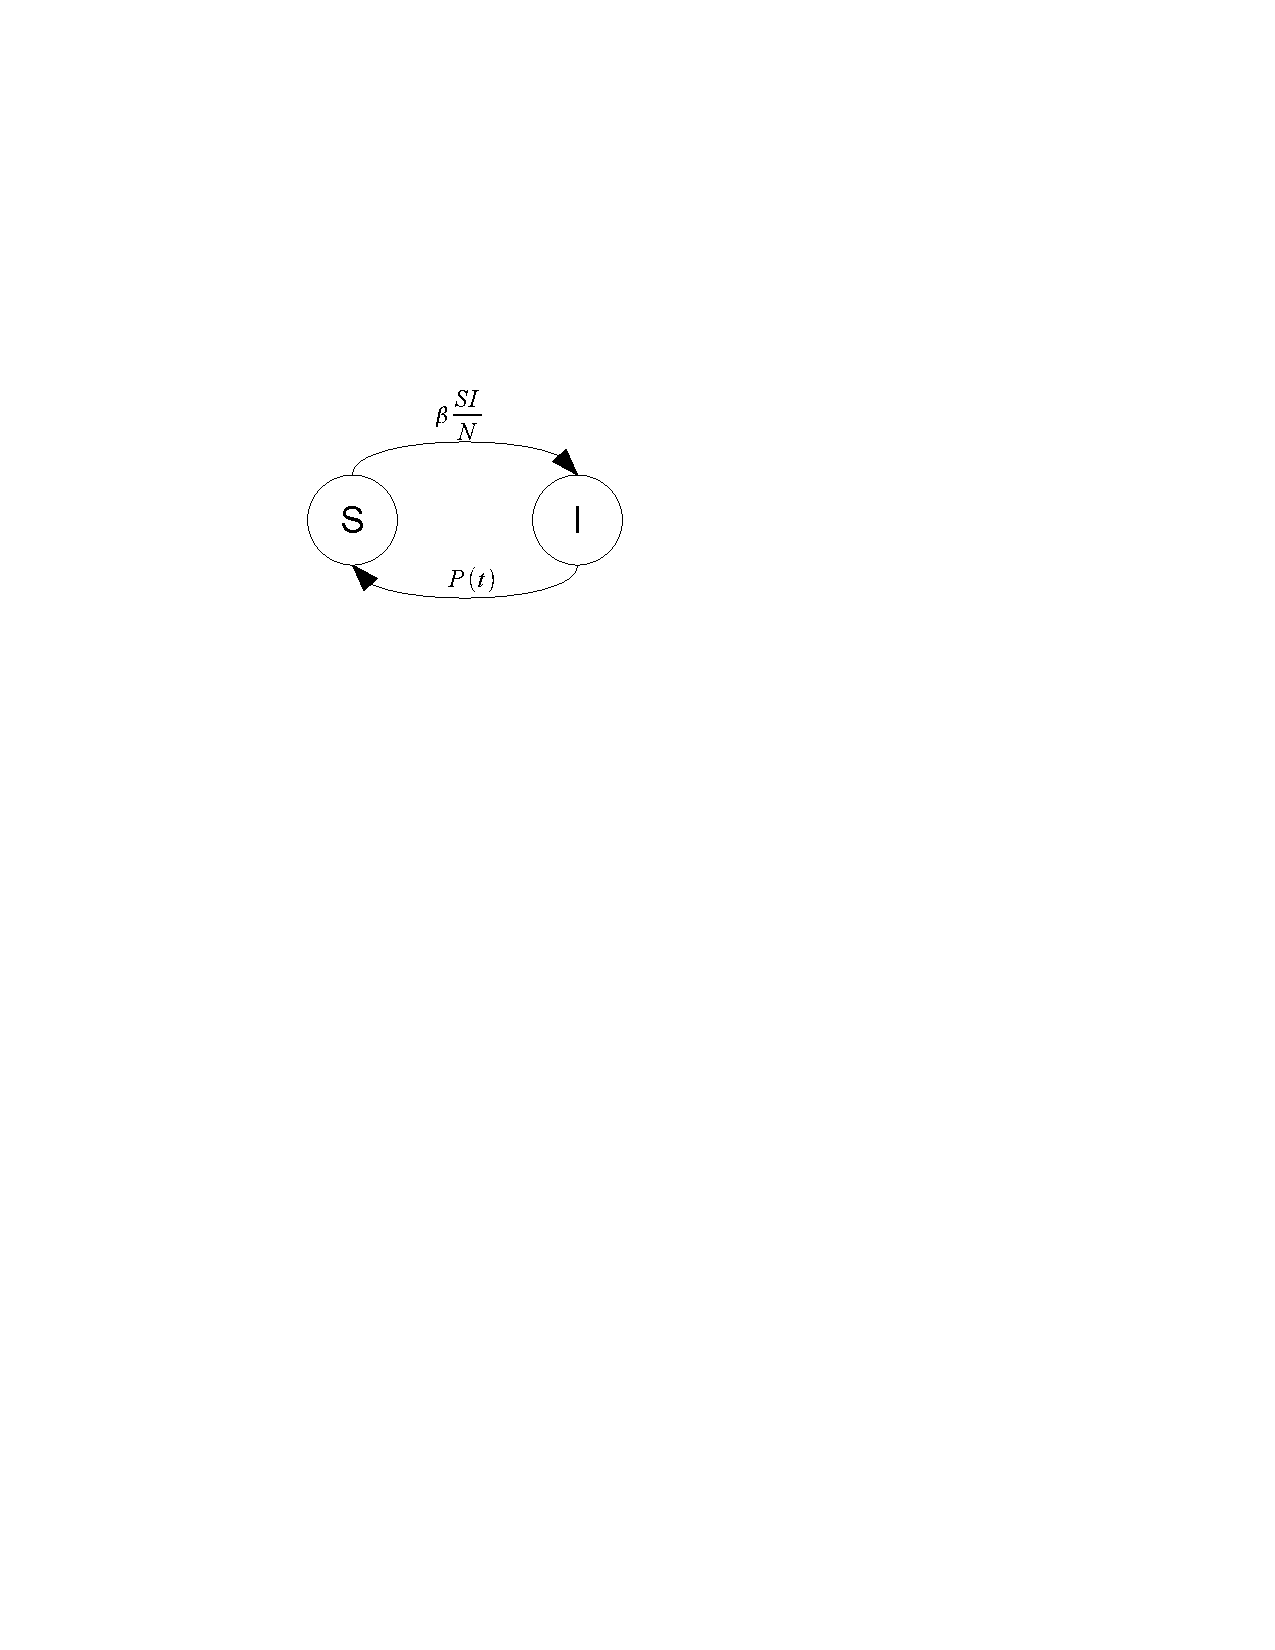
\includegraphics[width=0.45\textwidth]{../figs_03_residence_time/SIS_general}
\caption{The flow diagram of the model with arbitrary infectious period.}
\label{fig:flow_diagram_SIS_P}
\end{center}
\end{figure}
It details the flows of individuals between the compartments in the system.
It is extremely useful to rapidly understand what processes are modelled.


\frame{\frametitle{Reducing the dimension of the problem}
To formulate our model, we would in principle require an equation for $S$ and an equation for $I$.


But we have
\[
S(t)+I(t)=N, \textrm{ or equivalently, }S(t)=N-I(t).
\]
$N$ is constant (equal total population at time $t=0$), so we can deduce the value of $S(t)$, once we know $I(t)$, from the equation $S(t)=N-I(t)$.


We only need to consider 1 equation. {\bf Do this when possible!} (nonlinear systems are hard, one less equation can make a lot of difference)
}

\frame{\frametitle{Model for infectious individuals}
Integral equation for the number of infective individuals: 
\begin{equation}
I(t) = I_0(t)+ \int_0^t\beta\frac{(N-I(u))I(u)}{N} P(t-u) du
\label{eq:SIS_I} 
\end{equation}
\begin{itemize}
\item $I_0(t)$ number of individuals who were infective at time
$t=0$ and still are at time $t$.
\begin{itemize}
\item $I_0(t)$ is nonnegative, nonincreasing, and
such that $\lim_{t\to\infty}I_0(t)=0$.
\end{itemize}
\item $P(t-u)$ proportion of individuals who became infective at time $u$ and
who still are at time $t$.
\item $\beta (N-I(u))S(u)/N$ is $\beta S(u)I(u)/N$ with $S(u)=N-I(u)$, from the reduction of dimension.
\end{itemize}
}


\frame{\frametitle{Expression under the integral}
Integral equation for the number of infective individuals: 
\begin{equation}
I(t) = I_0(t)+ \int_0^t\beta\frac{(N-I(u))I(u)}{N} P(t-u) du
\tag{\ref{eq:SIS_I}} 
\end{equation}
The term
\[
\beta\frac{(N-I(u))I(u)}{N} P(t-u)
\]
\begin{itemize}
\item $\beta (N-I(u))I(u)/N$ is the rate at which new infectives are created, at time $u$,
\item multiplying by $P(t-u)$ gives the proportion of those who became infectives at time $u$ and who still are at time $t$.
\end{itemize}
Summing over $[0,t]$ gives the number of infective individuals at time $t$.
}


\frame{\frametitle{Case of an exponentially distributed time to recovery}
Suppose that $P(t)$ is such that the sojourn time in the infective
state has an exponential distribution with mean $1/\gamma$,
\emph{i.e.}, $P(t)=e^{-\gamma t}$.

Then the initial condition function $I_0(t)$ takes the form
\[
I_0(t)=I_0(0)e^{-\gamma t},
\]
with $I_0(0)$ the number of infective individuals at time $t=0$. This is obtained by considering the cohort of initially infectious individuals, giving a model such as \eqref{eq:N_general}.
Equation (\ref{eq:SIS_I}) becomes
\begin{equation}\label{eq:I_ODE}
I(t)=I_0(0)e^{-\gamma t}+\int_0^t \beta\frac{(N-I(u))I(u)}{N} e^{-\gamma (t-u)}du.
\end{equation}
Taking the time derivative of \eqref{eq:I_ODE} yields
\begin{align*}
I'(t) &= -\gamma I_0(0)e^{-\gamma t}-\gamma\int_0^t \beta\frac{(N-I(u))I(u)}{N}e^{-\gamma(t-u)}du +\beta \frac{(N-I(t))I(t)}{N} \\
&= -\gamma\left(I_0(0)e^{-\gamma t}+
\int_0^t \beta\frac{(N-I(u))I(u)}{N}e^{-\gamma(t-u)}du\right)+\beta \frac{(N-I(t))I(t)}{N} \\
&= \beta \frac{(N-I(t))I(t)}{N}-\gamma I(t),
\end{align*}
which is the classical logistic type ordinary differential equation
(ODE) for $I$ in an SIS model without vital dynamics (no birth or death).
}

\frame{\frametitle{Case of a step function survival function}
Consider case where the time spent infected has survival function 
\[
P(t)=\begin{cases}
1, & 0\leq t\leq\omega,\\
0, & t>\omega.
\end{cases}
\]
i.e., the sojourn time in the infective state is a constant
$\omega>0$.
 
In this case (\ref{eq:SIS_I}) becomes
\begin{equation}\label{eq:I_DDE}
I(t)=I_0(t)+\int_{t-\omega}^t \beta\frac{(N-I(u))I(u)}{N} du.
\end{equation}
Here, it is more difficult to obtain an expression for $I_0(t)$. It is however assumed that $I_0(t)$ vanishes for $t>\omega$.
}

\frame{
When differentiated, \eqref{eq:I_DDE} gives, for $t\geq\omega$,
\[
I'(t)=I_0'(t)+\beta\frac{(N-I(t))I(t)}{N}
-\beta\frac{\left(N-I(t-\omega)\right)I(t-\omega)}{N}.
\]
Since $I_0(t)$ vanishes for $t>\omega$, this gives the delay
differential equation (DDE)
\[
I'(t)=\beta\frac{(N-I(t))I(t)}{N}
-\beta\frac{(N-I(t-\omega))I(t-\omega)}{N}.
\]
}

\section{Conclusion}
\begin{itemize}
\item The distribution of the time of sojourn in classes (compartments) plays an important role in determining the type of model that we deal with.
\item All compartmental ODE models, when they use terms of the form $\kappa X$, make the assumption that the time of sojourn in compartments is exponentially distributed.
\item At the other end of the spectrum, delay differential equations with discrete delay make the assumption of a constant sojourn time, equal for all individuals.
\item Both can be true sometimes.. but reality is often somewhere in between. See Figure~\ref{fig:exp_distrib_80years} for an example of how an exponential distribution, with its fat tail, overepresents long sojourn times.
\end{itemize}

\begin{figure}[htbp]
\begin{center}
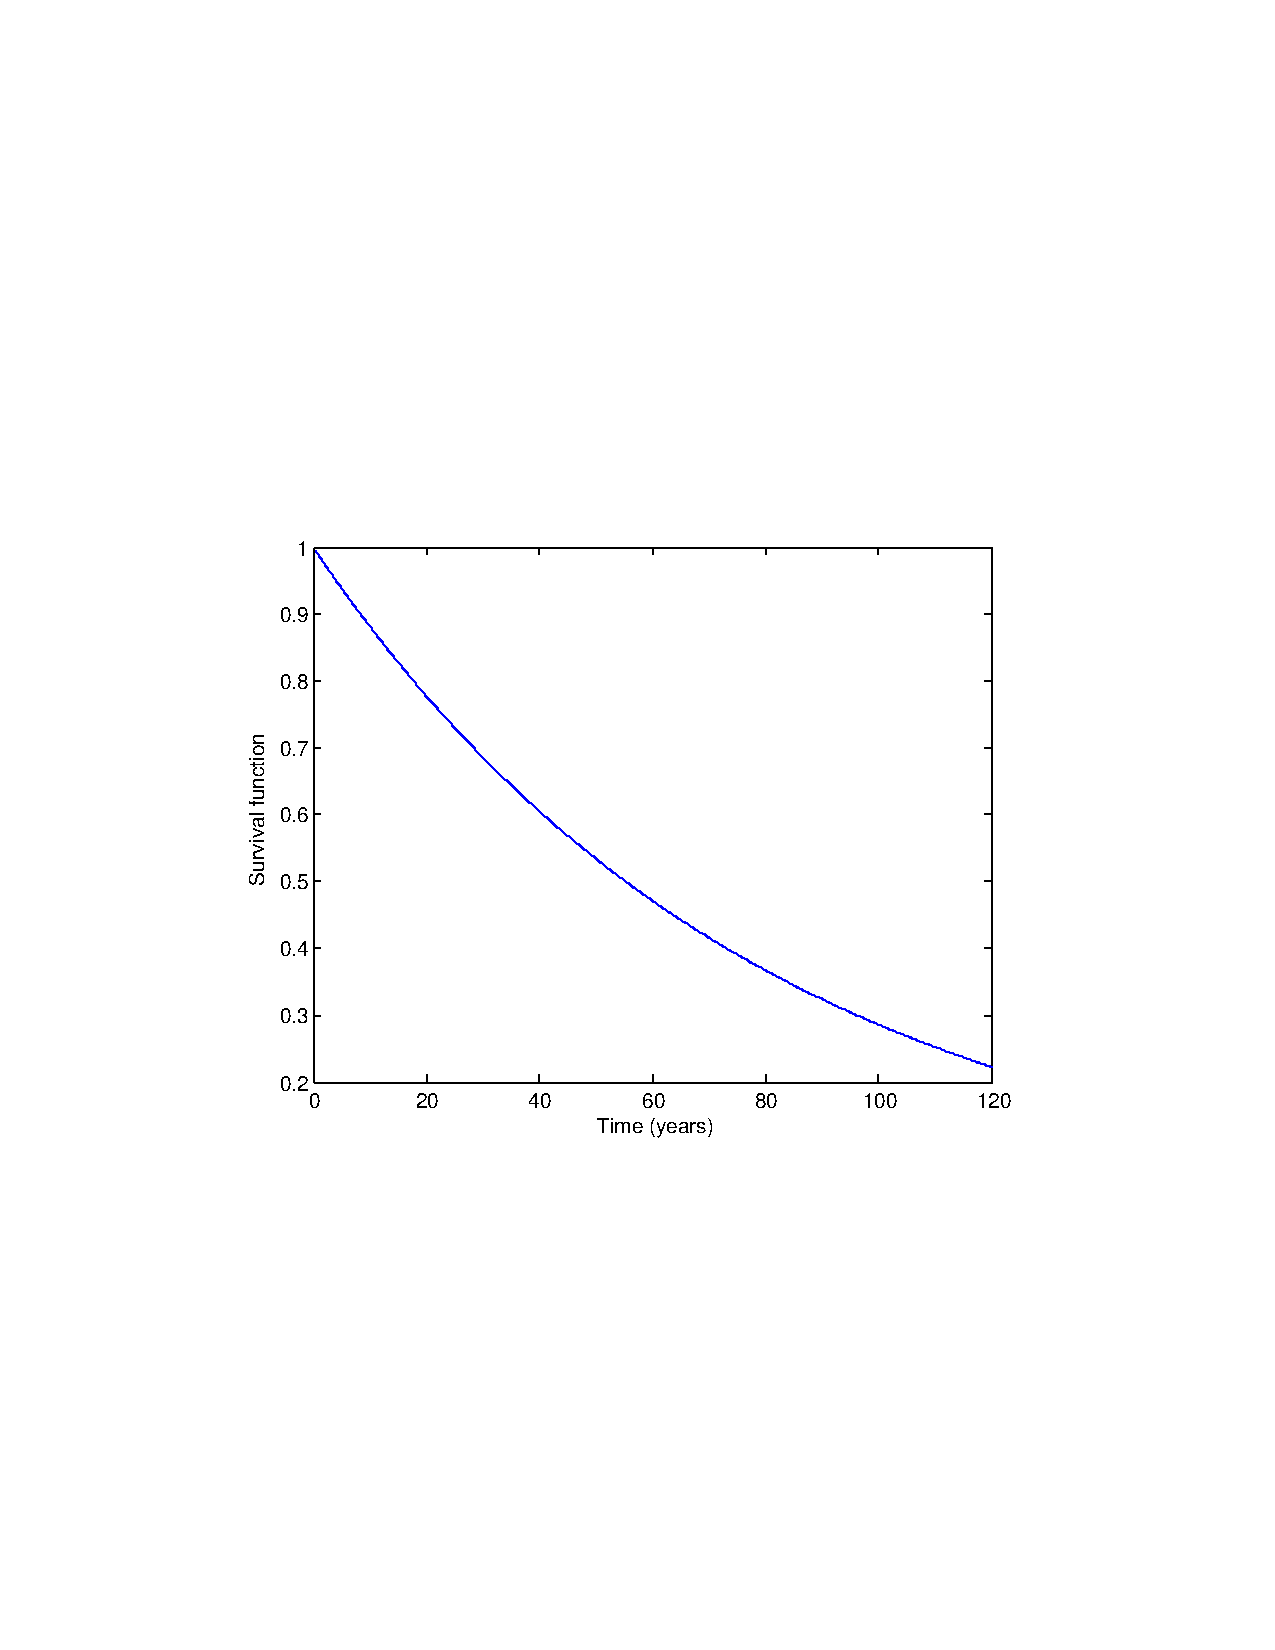
\includegraphics[width=0.5\textwidth]
{../figs_03_residence_time/survival_exp_80years}
\caption{Survival function, $\S(t)=\Proba{T>t}$, for an exponential distribution with mean 80 years. Note that this implies that more than 20\% of individuals in a cohort survive past the age of 120 years.}
\label{fig:exp_distrib_80years}
\end{center}
\end{figure}

%\frame{
%The \textbf{basic reproduction number}, denoted by $\Rzero$, which is a
%key concept in mathematical epidemiology, is now introduced. 
%It is defined as
%the expected number of secondary cases produced, in a completely
%susceptible population, by the introduction of a typical infective
%individual.  
%For this ODE model, $\Rzero=\beta/\gamma$.
%In terms of stability, the disease free equilibrium (DFE) with $I=0$
%is stable for $\Rzero<1$ and unstable for $\Rzero>1$. 
%At the threshold $\Rzero=1$, there is a forward bifurcation
%with a stable endemic equilibrium (with $I>0$) for $\Rzero>1$. Thus
%the value of $\Rzero$ determines whether the disease dies out or tends
%to an endemic value.
%}
